%%
%% This is file `sample-sigconf.tex',
%% generated with the docstrip utility.
%%
%% The original source files were:
%%
%% samples.dtx  (with options: `sigconf')
%% 
%% IMPORTANT NOTICE:
%% 
%% For the copyright see the source file.
%% 
%% Any modified versions of this file must be renamed
%% with new filenames distinct from sample-sigconf.tex.
%% 
%% For distribution of the original source see the terms
%% for copying and modification in the file samples.dtx.
%% 
%% This generated file may be distributed as long as the
%% original source files, as listed above, are part of the
%% same distribution. (The sources need not necessarily be
%% in the same archive or directory.)
%%
%% Commands for TeXCount
%TC:macro \cite [option:text,text]
%TC:macro \citep [option:text,text]
%TC:macro \citet [option:text,text]
%TC:envir table 0 1
%TC:envir table* 0 1
%TC:envir tabular [ignore] word
%TC:envir displaymath 0 word
%TC:envir math 0 word
%TC:envir comment 0 0
%%
%%
%% The first command in your LaTeX source must be the \documentclass command.
\documentclass[sigconf,nonacm]{acmart}
%% NOTE that a single column version may be required for 
%% submission and peer review. This can be done by changing
%% the \doucmentclass[...]{acmart} in this template to 
%% \documentclass[manuscript,screen]{acmart}
%% 
%% To ensure 100% compatibility, please check the white list of
%% approved LaTeX packages to be used with the Master Article Template at
%% https://www.acm.org/publications/taps/whitelist-of-latex-packages 
%% before creating your document. The white list page provides 
%% information on how to submit additional LaTeX packages for 
%% review and adoption.
%% Fonts used in the template cannot be substituted; margin 
%% adjustments are not allowed.
%%
%%
%% \BibTeX command to typeset BibTeX logo in the docs
\AtBeginDocument{%
  \providecommand\BibTeX{{%
    \normalfont B\kern-0.5em{\scshape i\kern-0.25em b}\kern-0.8em\TeX}}}

%% Rights management information.  This information is sent to you
%% when you complete the rights form.  These commands have SAMPLE
%% values in them; it is your responsibility as an author to replace
%% the commands and values with those provided to you when you
%% complete the rights form.
\setcopyright{acmcopyright}
\copyrightyear{2022}
\acmYear{2022}
\acmDOI{XXXXXXX.XXXXXXX}

%% These commands are for a PROCEEDINGS abstract or paper.
\acmConference[SCORES'22]{Student Computing Research Symposium}{October 6,
2022}{Ljubljana, Slovenia}
%
%  Uncomment \acmBooktitle if th title of the proceedings is different
%  from ``Proceedings of ...''!
%
%\acmBooktitle{Woodstock '18: ACM Symposium on Neural Gaze Detection,
%  June 03--05, 2018, Woodstock, NY} 
\acmPrice{15.00}
\acmISBN{978-1-4503-XXXX-X/18/06}


%%
%% Submission ID.
%% Use this when submitting an article to a sponsored event. You'll
%% receive a unique submission ID from the organizers
%% of the event, and this ID should be used as the parameter to this command.
%%\acmSubmissionID{123-A56-BU3}

%%
%% For managing citations, it is recommended to use bibliography
%% files in BibTeX format.
%%
%% You can then either use BibTeX with the ACM-Reference-Format style,
%% or BibLaTeX with the acmnumeric or acmauthoryear sytles, that include
%% support for advanced citation of software artefact from the
%% biblatex-software package, also separately available on CTAN.
%%
%% Look at the sample-*-biblatex.tex files for templates showcasing
%% the biblatex styles.
%%

%%
%% The majority of ACM publications use numbered citations and
%% references.  The command \citestyle{authoryear} switches to the
%% "author year" style.
%%
%% If you are preparing content for an event
%% sponsored by ACM SIGGRAPH, you must use the "author year" style of
%% citations and references.
%% Uncommenting
%% the next command will enable that style.
%%\citestyle{acmauthoryear}

\newcommand{\scores}{\textsc{SCORES}}
\renewcommand{\keywordsname}{Ključne besede}
\renewcommand{\acksname}{Zahvala}
\usepackage[slovene]{babel}
\usepackage{verbatim}
\usepackage{booktabs}
\usepackage[linesnumbered, boxed, resetcount]{algorithm2e}
\usepackage{hyperref}
\usepackage{hyperxmp}
\SetAlgorithmName{Algoritem}{Algoritem}

%%
%% If you need any other LaTeX packages, add them here
%%

%%
%% end of the preamble, start of the body of the document source.
\begin{document}

%%
%% The "title" command has an optional parameter,
%% allowing the author to define a "short title" to be used in page headers.
\title{Predloga za izdelavo prispevkov za SCORES v sistemu \LaTeX}


%%
%% The "author" command and its associated commands are used to define
%% the authors and their affiliations.
%% Of note is the shared affiliation of the first two authors, and the
%% "authornote" and "authornotemark" commands
%% used to denote shared contribution to the research.
\author{Kemen Berkovič}
%\authornote{Vsi trije avtorji so prispevali enakovreden dele\v{z}.}
\email{klemen.berkovic1@um.si}
\affiliation{%
    \institution{Faculty of Electrical \\Engineering and Computer Science,\\
    University of Maribor\\Koroška cesta 46}
    \city{SI-2000 Maribor}
    \country{Slovenia}
}

\author{Iztok Fister Jr.}
%\authornotemark[1]
\email{iztok.fister1@um.si}
\affiliation{%
    \institution{Faculty of Electrical \\Engineering and Computer Science,\\
    University of Maribor\\Koroška cesta 46}
    \city{SI-2000 Maribor}
    \country{Slovenia}
}

\author{Iztok Fister}
%\authornotemark[1]
\email{iztok.fister@um.si}
\affiliation{%
    \institution{Faculty of Electrical \\Engineering and Computer Science,\\
    University of Maribor\\Koroška cesta 46}
    \city{SI-2000 Maribor}
    \country{Slovenia}
}

\author{Luka F\"{u}rst}
\email{luka.fuerst@fri.uni-lj.si}
\affiliation{%
    \institution{Faculty of Computer and \\Information Science,\\
    University of Ljubljana\\Večna pot 113}
    \city{SI-1000 Ljubljana}
    \country{Slovenia}
}

%%
%% The abstract is a short summary of the work to be presented in the
%% article.
\begin{abstract}
    Pri"cujo"ci dokument podaja predlogo dokumenta v sistemu \LaTeX, ki
    ustreza slogovnim smernicam zbornika konference \scores\ in služi kot
    vodič k pripravi prispevka za to konferenco.  Avtorji so poskušali zajeti
    ve"cino pogosto uporabljenih elementov, kot so naslovi in podnaslovi,
    no"zne opombe, sklici, enačbe, tabele, slike, seznami, algoritmi itd.
    Izvorno kodo dokumenta (datoteko \texttt{.tex}) prevedite z ukazoma
    \texttt{pdflatex} in \texttt{bibtex} in dobljeni izhodni dokument
    (datoteko \texttt{.pdf}) primerjajte z referen"cnim.
\end{abstract}

%%
%% Keywords. The author(s) should pick words that accurately describe
%% the work being presented. Separate the keywords with commas.
\keywords{zbornik, \LaTeX, označevanje besedila\footnote{Navedite od tri do
deset ključnih besed, ki so specifične za vaš prispevek, a se znotraj
(o"zjega) podro"cja va"sega dela kljub temu pogosto uporabljajo.}}

%%
%% This command processes the author and affiliation and title
%% information and builds the first part of the formatted document.
\maketitle

\section{Uvod}

\emph{Zbornik} je zbirka prispevkov, predstavljenih na konferenci.
Organizacijski odbor konference \scores\ se trudi za slogovno poenotenost in
tipografsko kakovost prispevkov, zato dolo"ca nekaj strogih pravil za njihovo
oblikovanje.  Tako je med drugim predpisana osnovna oblika dokumenta
(dvostolp"cni format), pisava in njena velikost, dol"zina posameznih robov,
širina stolpca in razmak med stolpcema.

K sre"ci za vse našteto poskrbi sistem \LaTeX.  Avtorji se morate zgolj
dr"zati nekaj preprostih pravil in zagotoviti, da izhodni dokument PDF ne
presega \textbf{"stirih strani}.

V preostanku tega dokumenta predstavljamo izbor \LaTeX{}ovih ukazov za
dolo"citev zgradbe va"sega dokumenta.  Namesto da bi vsak ukaz posebej
natan"cno opisali ali pojasnili, smo se raje odlo"cili za predstavitev ukazov
s pomo"cjo primerov v kontekstu vzor"cnega dokumenta.

\section{\emph{Jedro} "clanka}

Jedro članka je obi"cajno organizirano v hierarhično strukturo z oštevilčenimi
ali neoštevilčenimi razdelki, podrazdelki, pod-podrazdelki itd.  Ukaz
\texttt{\textbackslash{}section} pred tem odstavkom je del take hierarhije.
Ob uporabi ustreznih ukazov sistem \LaTeX{} sam poskrbi za to, da so naslovi
pravilno oštevilčeni in ume"s"ceni.  Če želite, da je naslov neoštevilčen,
preprosto dodajte zvezdico k imenu ukaza.  Primeri oštevilčenih in
neoštevilčenih naslovov se bodo v tem dokumentu vseskozi
pojavljali.\footnote{To je druga opomba. Ne podaja ni"cesar vsebinskega,
temveč služi samo prikazu, kako delujejo in izgledajo opombe.  Opomba je
precej dolga, da lahko vidite, kako se takšna dolga opomba prikaže v kon"cnem
dokumentu.}

Ker je celoten članek vsebovan v okolju \textbf{document}, lahko začetek
novega odstavka označite z prazno vrstico (ta stavek je zato v novem odstavku).

\subsection{Spremembe pisave in \emph{posebni} znaki}

Nekaj sprememb pisave smo v tem dokumentu "ze videli.  V svojem besedilu lahko
besede ali besedne zveze z ukazom \texttt{\textbackslash{}emph} ali
\texttt{\textbackslash{}textit} prika"zete \emph{le"ze"ce}, z ukazom
\texttt{\textbackslash{}textbf} \textbf{krepko}, z ukazom
\texttt{\textbackslash{}texttt} pa \texttt{v slogu pisalnega stroja} (na
primer za programsko kodo).  Ne pozabite, da za spremembe pisave, ki so del
\emph{strukturnih elementov} (kot so na primer naslovi razdelkov), poskrbi
sistem sam.

V svojem dokumentu lahko uporabljate poljubne simbole, posebne znake
ali tuje znake.\footnote{Tretja opomba. Ta je precej kratka.} Seznam vseh
razpoložljivih simbolov najdete v \emph{\LaTeX{} User's
Guide}~\cite{Lamport:LaTeX}.

\subsection{Matematične enačbe}

Matematične enačbe lahko prikažete v treh različnih slogih:\ vrsti"cni (ang.\
\emph{inline}), oštevilčen blo"cni ali neoštevilčen blo"cni.  V naslednjih
razdelkih podrobneje obravnavamo vse naštete sloge.

\subsubsection{Vrsti"cne enačbe}

Enačba, ki se pojavi znotraj vrstice besedila, se imenuje vrsti"cna enačba.
Izdelamo jo z uporabo okolja \textbf{math}, ki ga lahko prikli"cemo z
obi"cajnim konstruktom
\texttt{\textbackslash{}begin}--\texttt{\textbackslash{}end} ali pa preprosto
z \textbf{\$$\ldots$\$}.  Uporabljate lahko katerekoli simbole in konstrukte,
ki so na voljo v sistemu \LaTeX~\cite{Lamport:LaTeX}, od $\alpha$ do $\omega$.

Vrsti"cni prikaz ni povsem enakovreden blo"cnemu. Na primer, kot bomo videli
v naslednjem razdelku, vrsti"cna enačba
\begin{math}\lim_{x\rightarrow \infty}\frac{1}{x}=0\end{math} 
v blo"cnem prikazu izgleda nekoliko druga"ce.

\subsubsection{Blo"cne enačbe}

Oštevilčeno blo"cno enačbo --- takšno, ki je navpično odmaknjena od besedila
in vodoravno poravnana --- izdelamo z uporabo okolja \textbf{equation}.
Neoštevilčene blo"cne enačbe vpeljemo z uporabo okolja \textbf{displaymath}.

Tudi v teh dveh okoljih uporabljate poljubne simbole in konstrukte, ki so na
voljo v sistemu \LaTeX. Ta odsek prikazuje zgolj nekaj primerov blo"cnih
enačb.

Najprej si oglejmo enačbo, ki je bila prej prikazana v vrsti"cnem načinu: 
%
\begin{equation}
\lim_{x\rightarrow \infty}\frac{1}{x}=0.
\end{equation}
%
Lahko vidimo, da je izgled v okolju \textbf{displaymath} drugačen od vrsti"cnega
prikaza.  Sedaj pa izdelajmo neoštevilčeno enačbo
%
\begin{displaymath}
    \sum_{i=1}^{\infty} \frac{1}{x^2} = \frac{\pi^2}{6},
\end{displaymath}
%
ki ji sledi še oštevilčena:
%
\begin{equation}
    \int_{0}^{\pi/2} \cos x\,dx = \sin x\bigg\rvert_{0}^{\pi/2} = \sin
    \frac{\pi}{2} - \sin 0 = 1.
\end{equation}

Sledi primer neoštevilčene enačbe, ki ni definirana v okolju
\textbf{displaymath}, temveč v kratki obliki (\textbf{\$\$$\ldots$\$\$}).  Ko $a
\ne 0$, ima enačba $ax^2 + bx + c = 0$ dve re"sitvi, in sicer:
%
$$x_{1, 2} = \frac{-b \pm \sqrt{b^2-4ac}}{2a}.$$

Oglejmo si "se primer sklicevanja na enačbo. Enačba~(\ref{equ:yannibel})
prikazuje, kako v sistemu \LaTeX{} zapisujemo pogoje.
%
\begin{equation}
    \begin{aligned} 
        \mathrm{nr}(G_i,r) & = \label{equ:yannibel}
        \begin{cases}
            1,  & \text{če $r$ igra en član iz $G_i$};\\
            -2, & \text{če $r$ ne igra nobeden član iz $G_i$}; \\
            -p, & \text{če $r$ igra $p$ članov iz $G_i$}.\\
        \end{cases}
    \end{aligned}
\end{equation}

\subsubsection{Dolge enačbe}

Kadar je enačba predolga za en stolpec, uporabite okolje \textbf{aligned}
znotraj okolja \textbf{equation}.  Za poravnavo ena"cbe v okolju
\textbf{aligned} uporabite znak \textbf{\&}, kot je razvidno iz
enačbe~(\ref{equ:ho}).
%
\begin{equation}
    \begin{aligned}
        O_{\max}& = w_1 \sum_{a=1}^{m} \sum_{b=a+1}^{n} (-\lvert\text{CPT}_a 
        -\text{CPT}_b\rvert)\\ 
        &\quad + w_2 \sum_{j=1}^{m} (\text{DIF}_j) + w_3 \sum_{j=1}^{m} 
        (\text{INT}_j/\sum_{x=1}^{n} x_{ij})
    \end{aligned}
    \label{equ:ho}
\end{equation}

\subsection{Citiranje}

V svojem "clanku boste najbr"z pogosto citirali članke \cite{lecun2015deep,
braams:babel, herlihy:methodology}, konferenčne zbornike
\cite{vrbancic2019transfer, clark:pct} ali knjige \cite{salas:calculus,
Lamport:LaTeX, fister2019computational}.  "Clanek se mora zaklju"citi s
seznamom vseh citiranih del (razdelek Bibliografija).  Tega seznama nikar ne
izdelujte ro"cno, pa"c pa uporabite ukaz \texttt{bibtex}.  Pri vsakem sklicu
na bibliografski vir morate zgolj uporabiti enega od ukazov za citiranje.
Ukazu kot parameter podate oznako, ki vir enoli"cno dolo"ca (t.i.\ klju"c
vira).  V tem dokumentu za ključ uporabljamo avtorjev priimek in besedo iz
naslova vira.  Ključ vira je definiran pri vsakem vnosu v datoteki
\texttt{.bib} vašega članka.

Podrobnosti ustvarjanja datoteke \texttt{.bib} presegajo okvir tega dokumenta.
Več informacij lahko najdete v \emph{Author's Guide} in \emph{\LaTeX{} User's
Guide} \cite{Lamport:LaTeX}.

V pri"cujo"cem dokumentu uporabljamo samo najosnovnejši ukaz za citiranje
(\texttt{\textbackslash{}cite}).  Ta na"cin je dejansko edini, ki je skladen s
smernicami v specifikacijah ACM\@.

\subsection{Tabele}

Ker tabele ni mogoče razdeliti na več strani, jo obi"cajno umestimo na vrh
strani v bli"zino prvega sklica nanjo.  Da zagotovite pravilno umestitev in
poravnavo tabel, uporabite okolje \textbf{table} in vanj postavite vsebino in
naslov tabele.  Sama vsebina tabele se mora nahajati znotraj okolja
\textbf{tabular}, ki poskrbi za pravilno poravnavo vrstic in stolpcev.
Podrobnejša navodila so ponovno dostopna v \emph{\LaTeX{} User's Guide}.
    
Tabela~\ref{tab:table1} je vstavljena takoj za tem odstavkom.  Primerjajte
umestitev tabele znotraj izvorne datoteke z umestitvijo znotraj izhodnega
dokumenta PDF\@.

\begin{table}
    \centering
    \caption{Frekvence posebnih znakov.}
    \label{tab:table1}
    \begin{tabular}{ccl}
        \toprule
        Simbol&Frekvenca&Komentar\\
        \midrule
        \O & 1 na 1,000& Švedska imena.\\
        $\pi$ & 1 na 5& V matematiki.\\
        \$ & 4 na 5 & V ekonomiji.\\
        $\Psi^2_1$ & 1 na 40,000& Nepojasnjeno. \\
        \bottomrule
    \end{tabular}
\end{table}

Če želite širšo tabelo (tak"sno, ki zavzame celotno širino delovnega območja
na strani), uporabite okolje \textbf{table*}.  Kot pri tabeli z enim stolpcem
bo tudi ta samodejno umeščena na ustrezno mesto.  Tabela~\ref{tab:table2} je
vstavljena takoj za tem stavkom; vnovi"c primerjajte umestitev tabele v
izvorni datoteki z umestitvijo v izhodnem dokumentu PDF\@.

\begin{table*}
    \centering
    \caption{Nekaj tipičnih ukazov.}
    \label{tab:table2}
    \begin{tabular}{ccl}
        \toprule
        Ukaz&Numerična vrednost&Komentar\\
        \midrule
        \texttt{\textbackslash{}imagespath} & 200 & Mapa, kjer se nahajajo slike dokumenta. \\
        \texttt{\textbackslash{}table} & 300 & Za tabele.\\
        \texttt{\textbackslash{}table*} & 400& Za široke tabele.\\
        \bottomrule
    \end{tabular}
\end{table*}

\subsection{Slike}

Tako kot tabele se tudi slike ne morejo raztezati prek ve"c strani. Tudi slike
je najbolje umestiti na vrh ali dno strani v bli"zino prvega sklica
nanje.\footnote{Četrta (in zadnja) opomba.}  Da zagotovite ustrezno umestitev,
uporabite okolje \textbf{figure} ter vanj postavite sliko in njen opis.

Na sliki~\ref{fig:circles} je prikazana datoteka v formatu PDF, na
sliki~\ref{fig:star} pa datoteka v formatu PNG\@.

\begin{figure}
    \centering
    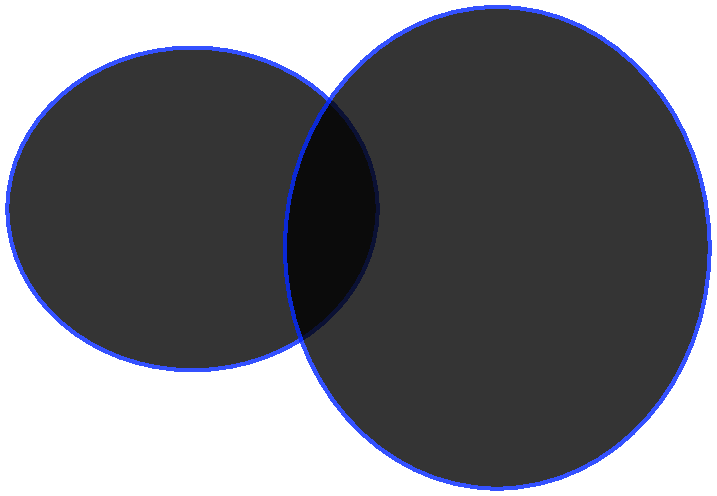
\includegraphics[scale=0.5]{circles.pdf}
    \caption{Krogi (format PDF).}
    \label{fig:circles}
\end{figure}

\begin{figure}
    \centering
    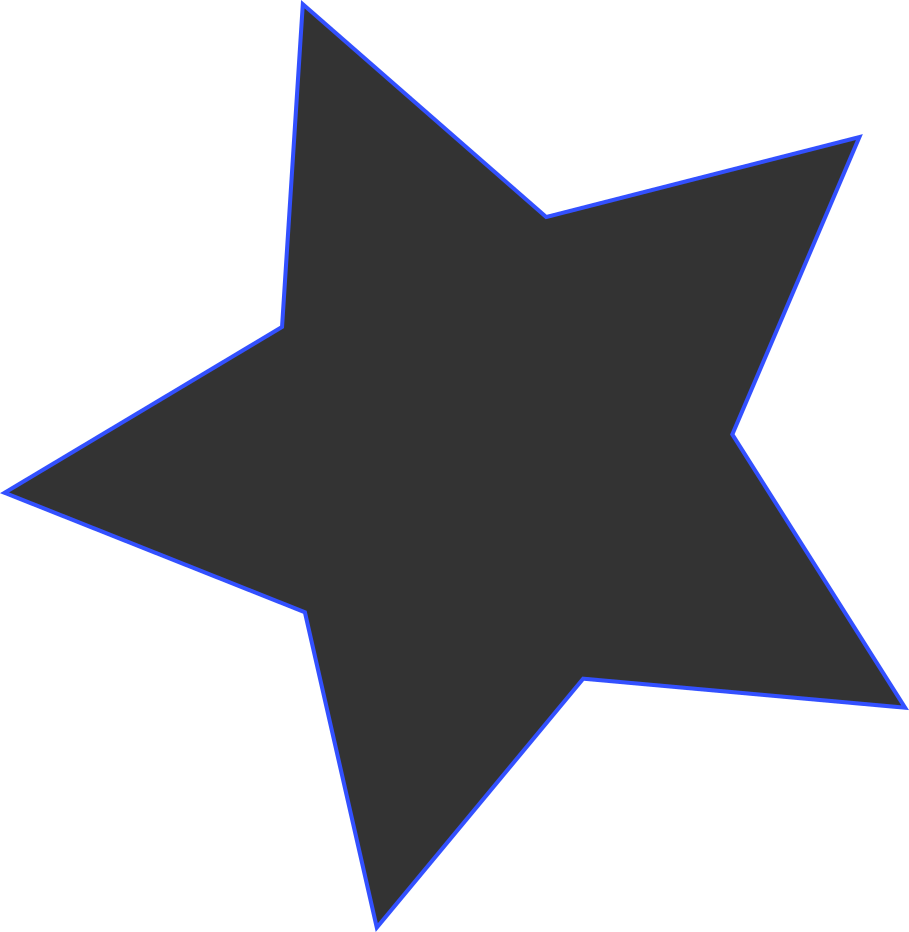
\includegraphics[scale=0.5]{star.png}
    \caption{Zvezda (format PNG).}
    \label{fig:star}
\end{figure}

Tudi slike se lahko raztezajo čez oba stolpca.  To lahko dose"zete z uporabo
okolja \textbf{figure*}.  Tak primer prikazuje slika~\ref{fig:spin}.

\begin{figure*}
    \centering
    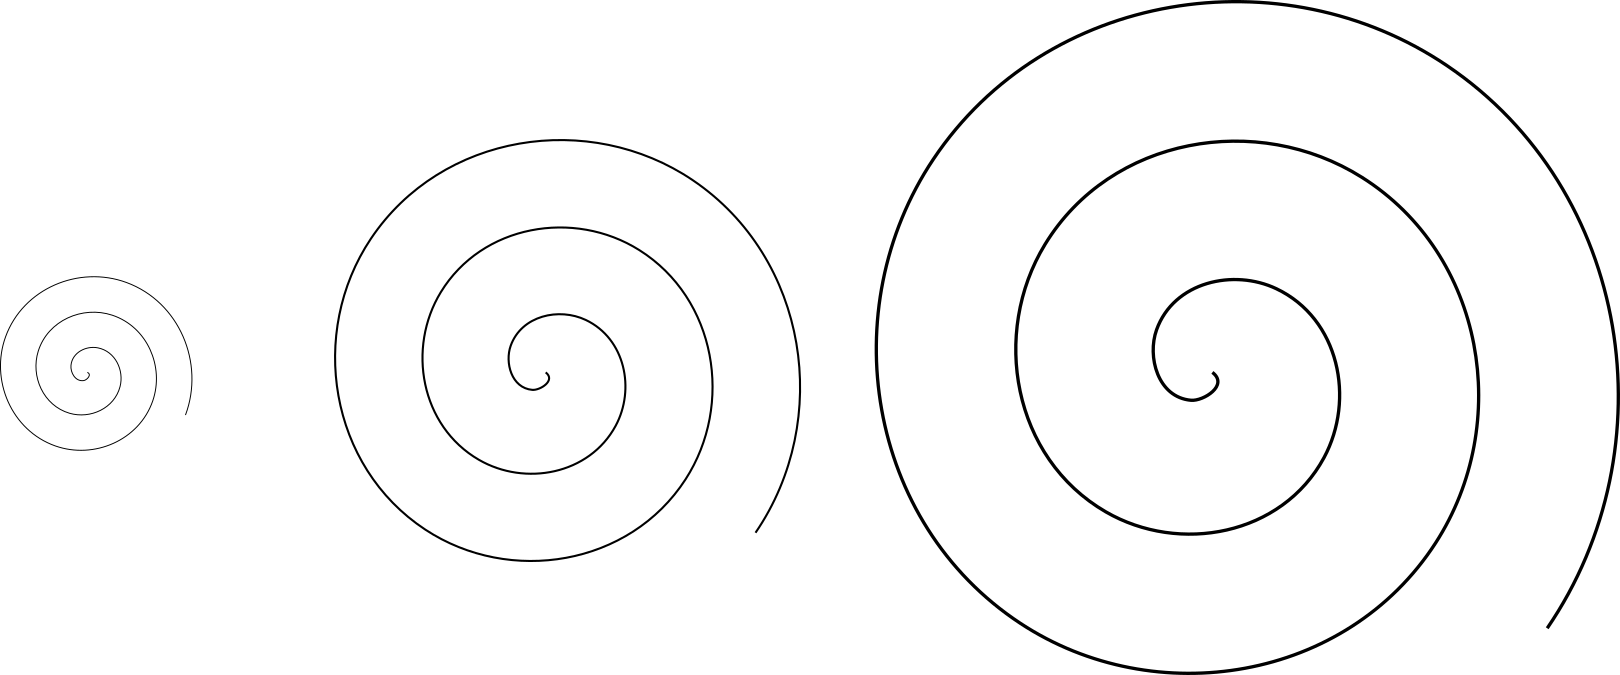
\includegraphics[scale=0.8]{spin.png}
    \caption{Slika, ki se razteza "cez oba stolpca.}
    \label{fig:spin}
\end{figure*}

\subsection{Seznami}

"Ce "zelite svoje ideje predstaviti po postavkah, uporabite seznam.  Seznam
ustvarite s pomo"cjo okolja \textbf{itemize}.  Oglejmo si primer:

\begin{itemize}
    \item prvi element,
    \item drugi element in
    \item tretji element.
\end{itemize}

Včasih se avtorji želijo sklicevati na posamezne postavke seznama.  V ta namen
lahko uporabite okolje \textbf{enumerate}, ki proizvede o"stevi"cem seznam.
Na primer:

\begin{enumerate}
    \item prva točka,
    \item\label{list:item} druga točka,
    \item \ldots
\end{enumerate}

Postavka \ref{list:item} nam pove, "cesa se moramo lotiti, ko odkljukamo
predhodno postavko.

\subsection{Algoritmi}

Če želite v svojem prispevku prikazati algoritem, uporabite okolje
\textbf{algorithm}.  Na algoritme se lahko sklicujemo na podoben na"cin kot na
tabele in slike (npr.\ algoritem~\ref{algo:sample}).

\begin{algorithm}
    \SetAlgoLined
    \KwData{tukaj je tekst}
    \KwResult{kako pisati algoritme v sistemu \LaTeX}
    inicializacija\;
    \tcc{tukaj se pri"cne glavni del kode}
    \While{ni konec dokumenta}{\label{algo:sample:while}
        preberi del dokumenta\;
        \eIf{razumeš}{
            pojdi na naslednji razdelek\;
            ta razdelek postane trenutni razdelek\;
        }{
            vrni se na začetek trenutnega razdelka\;
        }
    }
    \caption{Kako pisati algoritme.}
    \label{algo:sample}
\end{algorithm}

Kot je razvidno iz naslednjega stavka, se lahko sklicujete tudi na posamezne
vrstice algoritma.  Primer zanke \textbf{while} je viden v
vrstici~\ref{algo:sample:while}.

Podrobnejša navodila glede okolja
\textbf{algorithm} lahko najdete v dokumentu
\url{http://tug.ctan.org/macros/latex/contrib/algorithm2e/doc/algorithm2e.pdf}.

\section{Zaključek}

Ta odstavek končuje jedro tega vzorčnega dokumenta.  Morda boste dodali še
zahvalo (kratek primer sledi v nadaljevanju).  Urediti morate tudi
bibliografijo.  Za konec naj povemo, da so bibliografske enote, navedene v tem
dokumentu, z izjemo knjige o sistemu \LaTeX{} povsem nepovezane z obravnavano
temo in slu"zijo zgolj kot primeri.

\begin{acks}
    Ta razdelek ni obvezen.  Na tem mestu se lahko zahvalite za morebitna
    sredstva, financiranja, pomoč ali kaj drugega.
\end{acks}

\bibliographystyle{ACM-Reference-Format}
\bibliography{bibliografija}

\end{document}
